\chapter{Analysis and Discussion}\label{discussion}
This chapter will summarize the key findings presented in \Cref{experiments} and analyze them with respect to the theory as outlined in \Cref{background}. The limitations of the respective experiments will also be discussed, along with presenting potential directions of further research. The chapter will be organized according to the experiments performed, with each section discussing the results, implications, impact, and limitations of the corresponding experiment, as well as highlighting potential improvements and further work as informed by the findings for the given experiment. The chapter will start with the analysis of the impact of model architectures on generalization as presented in \Cref{models}, then moving on to the impact of augmentation as presented in \Cref{augmentations}, inconsistency training as presented in \Cref{consistency_training}, and finally ensembles as presented in \Cref{ensembles}. Finally, the last section will discuss miscellaneous ideas for directions of further research on generalizability which due to a variety of reasons were not explored in this thesis. 


\section{Model Architectures and Generalizability}
The experiments performed in \Cref{models} show that every model exhibited comparable levels of generalisation failure, with the exception of TriUnet which seemed to struggle more than any of the other models. On Etis-LaribDB, which evidently proved to be the most difficult dataset, every model exhibited a generalizability gap of at least around 50\%, with the TriUnet ranging upwards of 65\%. The degree of generalization failure was slightly less pronounced on the two other datasets, with CVC-ClinicDB exhibiting average gaps of approximately 18\% and EndoCV2020 25\%. 

The models exhibited comparable performance also in \gls{ind} settings, spanning between IoUs of 0.819 and 0.832, which for practical purposes can be considered negligible. 

\subsection{Impact}
Naturally, deploying any of the predictors from this experiment in a clinical setting would be inadvisable and perhaps even harmful. Even if the predictors were to be trained on a dataset collected exclusively from the centre they were intended to be deployed on, there is no guarantee that there would never be some form of distributional shift, which as evidenced by the results significantly affect performance. This distributional shift may be as simple as a change in endoscopy preparation routines, or perhaps an upgrade to a higher resolution cameras, and so on. As established in \Cref{background}, a system based on models with this lack of generalizability would be practically useless. 

Moreover, these results highlight that researching the development of more and more complicated task-agnostic models is a comparatively fruitless affair. The difference between DeepLabV3+ and Unet - which are separated by two years of research - are practically inconsequential. Admittedly, the differences are more pronounced when the models are trained according to the more sophisticated training regiments used in the remaining experiments, but it is nonetheless clear that it is not advancement in model architectures that is likely to result in increased generalization, but rather improvements to the pipeline with which they are trained.
\subsection{Dual Decoder Models}
\Cref{methods} introduced the dual-decoder DeepLabV3+, the intent of which was to increase generalization by constraining the space of latent representations that the model could leverage, thus in theory mitigating underspecification. As the results in \Cref{dd-deeplab} showed, however, the effect of this additional encoder was fairly limited when compared to the regular DeepLabV3+. Though it was argued that the reduced performance variability of the dual-decoder model could be interpreted as evidence for a reduction in underspecification, the performance in terms of mean IoU was identical across both models for practical purposes. It was hypothesized that this may be due to the encoder learning principally dataset-agnostic features and consequently primarily performing image compression regardless of what object the model is intended to segment. This was to some extent was corroborated by the analysis performed in \Cref{dd-deeplab}, which showed equivalent image reconstruction performance across datasets in terms of L1 distance. Further research is however required, as these findings are only representative of one specific model trained in a limited number configurations. One possible direction is to implement a wide range of encoder-decoder models trained across multiple decoder configurations and datasets, and then investigate the latent spaces of the resulting predictors. If the predictor encoders indeed do encode primarily dataset-agnostic features independent of the decoder function, one would expect that one could simply switch encoders between predictors trained on different datasets, domains and tasks without significant performance degradation. 

This behaviour may also be attributed to pretraining. Since the models used throughout this thesis were at least partially pretrained on Imagenet, it might simply be the case that the encoders have learned to perform image compression as a direct consequence of the fact that this likely is the most conducive configuration to minimizing risk on the Imagnet dataset. In this case, the encoder may be in such a wide minimum that actually learning domain-specific features is unlikely even after training to segment polyps. This will be discussed further in \Cref{pretraining}.


\section{Augmentation and Generalizability}
The experiment in \Cref{augmentations} demonstrated the efficacy of data augmentation as a means of increasing generalization, with IoU improvements on Etis-LaribDB averaging about 15\% and ranging upwards of 30\%. This, as mentioned in \Cref{background}, can be attributed to the increase in support that the wider diversity of data provides. 

\subsection{Impact}

What is surprising is the extent to which augmentation improves generalization in comparison to some of the other tested methods. In particular, the effects of model architectures and ensembles were both comparatively minuscule. The use of ensembles, for instance, the use of which was the basis of several of the papers submitted to EndoCV2021, increased generalization by at most \(PLACEHOLDER\%\) and on average \(PLACEHOLDER\%\) when consisting of predictors trained without augmentation at most \(PLACEHOLDER\%\) and on average \(PLACEHOLDER\%\) with augmentation, and finally at most \(PLACEHOLDER\%\) and on average \(PLACEHOLDER\%\) on consistency training. The use of data augmentation, on the other hand, led to increases of at most \(PLACEHOLDER\%\) and on average \(PLACEHOLDER\%\), and consistency training at most \(PLACEHOLDER\%\) and on average \(PLACEHOLDER\%\). What this means, in effect, is that the margins by which the use of augmentation affects generalization are far greater than the margins by which ensembles and perhaps many of the other methods presented in EndoCV2021 affect generalization. This raises questions as to the validity of the results in EndoCV2021, which did not control for the choice of data augmentations when comparing submissions. It may, for instance, be the case that certain submissions exhibited high degrees of generalization not strictly because of the impact of their proposed methods, but rather due to their choice of augmentations. This is of course not a certainty, and does as such warrant further research for instance in the form of a meta-analysis. 

\subsection{Inpainting and Generative Modelling}

The experiments in \Cref{augmentations} showed that the use of an inpainter as implemented in this thesis harmed generalization when used in conjunction with conventional augmentations. Two hypotheses for why this is the case were suggested - either the inpainter simply does not perform to a sufficient standard conducive for use as augmentation, or the inpainter learned the distribution to such an extent that it increased the models' dataset bias. 

To investigate this, it is possible to implement one of the more state-of-the-art inpainting architectures, for instance an inpainting generative multi-column network \cite{inpainter_better}. Additionally, analyzing the generated polyps via statistical means may also have some merit. The development of distance metrics to facilitate easier comparison between synthetic images to real images may for instance be worth looking into, as this might shed some light on the hypotheses as presented above.

\subsection{Limitations}
    Ignoring the inpainter and its flaws as outlined above, only one implementation of data augmentation was used throughout this thesis. The constituent transformations and the values of the hyperparameters thereof were also selected with limited prototyping or testing. There may as such be augmentation configurations that induce significantly increased generalization. By the same token, the selection of transformations used in this thesis may instead have been lucky and thus over-represent the typical contribution of data augmentation. A robust investigation of data augmentation and its effects would require a larger range of augmentation strategies. The results thereof would, however, only be of relevance to the particular task that is being considered. Polyp segmentation may benefit more from augmentation than image-captioning, for instance. 
    
    Additionally, the augmentations in this thesis were applied according to a predetermined probability. A more effective technique may be to augment every sample, but account for the severity through the modulation of the hyperparameters of the constituent transformations. This was not, however, investigated in this thesis, as the probability-based implementation facilitated more apples-to-apples comparison to consistency training. 

\section{Consistency Training}
Consistency training was shown to improve generalizability, outperforming data augmentation by a significant margin on Etis-LaribDB. As discussed in \Cref{methods}, this can be attributed to the fact that, in addition to increasing the models' support, similar to data augmentation, it also imposes more credible inductive biases by explicitly optimizing for consistency across augmentations. 


% \subsection{Mathematical Analysis of Consistency Training}
% The relationship between consistency training and conventional data augmentation may be more readily understood mathematically. As mentioned in \Cref{methods}, one can argue that they may be equivalent, but as the analysis below will show, this is not the case. To illustrate, consider the impact of the respective methods on the gradients. As discussed in \Cref{background}, the gradient simply defines a direction in the search landscape, and thus if it can be proved that the gradients are not equal (up to scale), it follows that the training process will explore different parts of the search-landscape, irrespective of any amount of tuning of learning rates or any of the other hyperparameters governing the optimization process. 

% As \gls{sil} is based in part on the Jaccard index, it will be compared to a pipeline that uses the Jaccard loss. Moreover, since data augmentation is a stochastic process - in other words, the augmentations applied according to some probability \(p\), the gradients can only be analyzed sufficiently by considering the expected loss. 
% \begin{align*}
%     \mathcal{L} &= \mathbb{E}_p[\mathcal{J}(Z)]; Z \in_{R \thicksim p} \{ \{y, \hat{y}\},\{a, \hat{a}\}\\
%     &= p\mathcal{J}(a, \hat{a})+ (1-p)\mathcal{J}(y, \hat{y})
% \end{align*}
% Thus, the expected gradient is simply:
% \begin{equation}
%     \nabla \mathcal{L} = p \nabla \mathcal{J}(a, \hat{a})+ (1-p)\nabla \mathcal{J}(a, \hat{a})
% \end{equation}
% In the case of \gls{sis}:
% \begin{align*}
%     \bar{\mathcal{C}} &= \sum \frac{\Theta(y, \hat{y},  a, \hat{a})}{\bigcup(y, \hat{y},  a, \hat{a})}\\
%     &= \sum \frac{\bigcup(\Theta(y, \hat{y}), \Theta(a, \hat{a}))- \bigcap (\Theta(y, \hat{y}), \Theta(a, \hat{a})) }{\bigcup(y, \hat{y},  a, \hat{a})}
%     &=...\\
%     \nabla \bar{\mathcal{C}} &=\frac{\mathrm{\nabla_{f}}\! \left(\Theta(y, \hat{y}) \right) \Theta(a, \hat{a})}{-\Theta(y, \hat{y}) \Theta(a, \hat{a}) +\Theta(a, \hat{a}) +\Theta(y, \hat{y})}+\\
%     &\frac{\Theta(y, \hat{y}) \mathrm{\nabla_{f}}\! \left(\Theta(a, \hat{a}) \right)}{-\Theta(y, \hat{y}) \Theta(a, \hat{a}) +\Theta(a, \hat{a}) +\Theta(y, \hat{y})}-\\&\frac{\Theta(y, \hat{y}) \Theta(a, \hat{a}) \left(-\mathrm{\nabla_{f}}\! \left(\Theta(y, \hat{y}) \right) \Theta(a, \hat{a}) -\Theta(y, \hat{y}) \mathrm{\nabla_{f}}\! \left(\Theta(a, \hat{a}) \right)+\mathrm{\nabla_{f}}\! \left(\Theta(a, \hat{a}) \right)+\mathrm{\nabla_{f}}\! \left(\Theta(y, \hat{y}) \right)\right)}{\left(-\Theta(y, \hat{y}) \Theta(a, \hat{a}) +\Theta(a, \hat{a}) +\Theta(y, \hat{y}) \right)^{2}}
% \end{align*}
% At this point, the expression is a bit unwieldy. However, it is worth noting that 
% TODO: finish typesetting remainding proof

% The gradients for the respective methods can then be expressed as follows:
% \begin{align}
%     \nabla \bar{C} &= \\
%     \nabla A &= \\
% \end{align}
% Though both are indeed merely weighted sums of the Jaccard losses for the augmented and unaugmented sets, the difference in how they are weighed is key. In contrast to conventional data augmentation, consistency training adjusts the loss dynamically according to segmentation performance. This fact may be used to facilitate the implementation consistency training also on other domains than segmentation, by instead modifying augmentation probabilities dynamically. This is left as a point of further research, along with investigating other improvements to consistency training as will be outlined in the following section. 


        
    \subsection{Impact}
    Though consistency training did increase generalization by a considerable amount, the \gls{ood} performance is nevertheless insufficient for practical purposes. The best performance on Etis-LaribDB with consistency training was after all merely 0.504, as shown in \Cref{tab:consistency}. This kind of performance would naturally be of limited utility in clinical applications. 
    
    Consistency Training does, however, constitute a step in the right direction. Given further development, it may in time prove a promising candidate as a means of alleviating generalization failure to practically viable extents. As established in \Cref{methods}, the limits are in theory only the efficacy of the quantification of consistency for a given task as well as the support provided by the augmentation strategy upon which it is based. Improvements to either of these aspects are likely to contribute to considerable gains in generalizability. 
    
    Developing perturbation models and consistency metrics may also be a great opportunity to incorporate expert input. A clinician could for instance offer insights as to the nature of the perturbations one might expect in practice and thus assist in the development of the perturbation model.
    
    

\subsection{Limitations}
    During the experiments performed in this thesis, the batch size was set to 8 for all training procedures. As consistency training relies on generating pairs of data from a given batch, one may argue that keeping the batch size the same may result in a weak comparison. The experiment should as such ideally be repeated across a number of batch sizes, but this was infeasible due to logistical constraints, in particular with regards to computational resources. 

    \subsection{Improving Consistency Training} \label{new_closs}
    As was shown in \Cref{experiments}, consistency training is an effective means of increasing generalization. However, there is still room for further improvement and exploration. For instance, in this thesis consistency was expressed merely as the symmetric difference between the expected change in the output due to augmentation and the actual change due to augmentation. This, however, as discussed in \Cref{methods}, is largely agnostic to the augmentation being performed. However, the nature of these augmentations should be taken into account. If the image is subjected to a 90 degree rotation, for instance, the prediction would be considered perfectly consistent so long as the pixels corresponding to the polyps are rotated, and the incorrectly classified pixels remain unchanged. However, if the model instead learns to rotate all of the pixels - even those that are incorrectly classified - it may learn a more accurate representation of what constitutes consistent behavior. I.e, instead of expressing inconsistency as:
    \begin{equation*}
        \bar{\mathcal{C}} = y\ominus a \ominus \hat{y} \ominus \hat{a}  
    \end{equation*}
    One can adjust the expected change term such that also incorrect predictions can be considered consistent so long as they change in accordance to the nature of the perturbation model \(\epsilon(\cdot)\):
        \begin{equation*}
        \bar{\mathcal{C}} = \hat{y}\ominus \hat{a} \ominus \hat{y}\ominus \epsilon(\hat{y})  
    \end{equation*}
    This also has the advantage of being independent of the labels themselves. This may alleviate complications that may arise as a consequence of poor and/or incomplete labeling which would otherwise affect what the models learn to associate with consistent behaviour. 

    In addition to improving the way by which consistency is quantified, there are several unexplored directions through which the training procedure itself could be further improved. The perturbation model, for instance, could be modified in any number of ways: one could for instance adversarially sample difficult augmentations based on the consistency score, and use these during training. One could also perform a study to ascertain the impact of the perturbation models' constituent augmentation functions on generalization. It may for instance be the case that some of the augmentations used in the perturbation model used in this thesis hampered generalizability more than it facilitated it, though without a complete study this is impossible to say with any certainty.  
    
    Moreover, one could experiment with modulating the difficulty of the augmentations. In the experiments performed in this thesis, the augmentation difficulty was kept constant - i.e, the augmentation hyperparameters were capped to a specific range. However, it may be the case that gradually increasing the difficulty or modulate it according to some sort of annealing function could further improve the efficacy of consistency training.    
\section{Ensembles and Generalizability}
    The use of ensembles, as shown in \Cref{ensembles}, proved to increase generalization. However, the notion that this improvement arises as a result of mitigating underspecification was shown to not be as strong as the analyses in the literature often suggest. 
    
    \subsection{Impact}
    The improvements due to the use of ensembles was, however, somewhat minor. As discussed in previous sections, data augmentation and consistency training proved to be more effective by significant margins. On the Etis-LaribDB dataset, conventional data augmentation provided improvements to generalization ranging between 10\% and 20\%, and consistency training between 20\% and 26\% when averaging across models. Ensemble models, on the other hand, ranged between actually harming generalization by a minor amount and at best facilitating a 13\% increase on the TriUnet.  The potential gains from ensemble models is nevertheless significant, but it should be noted that the ensembles' cost of training time, time required for inference, and the comparatively high memory requirements needs to be weighted against the benefits. It may, for instance, be the case that the computational resources spent training multiple models for use in an ensemble would be better spent tuning the augmentation strategy, which as established has a more considerable effect. 

    \subsection{Limitations}
    It should be noted that the experiments in this thesis were performed only at one ensemble size - i.e, 5 models. This choice was informed by the literature, in particular the implementation of DivergentNet \cite{divergentnets}. Ensembles may as such have a greater impact than expected, dependent on the returns from increasing the model counts. Following the Bayesian perspective, increasing the model count should result in a better estimate of the Bayesian posterior, and thus lead to increased generalization. 
    
    ...     
    
    \subsection{Diversity Search for Ensembles}
    Though the analysis shown in \Cref{fig:ensemble_var} showed that ensembles do not appear to increase generalization by mitigating underspecification, there may yet be a relationship between ensembles and model-diversity that warrants further research. it may be possible that there is a relationship between ensembles and model diversity which warrants further study. In particular, it may be the case that training multiple predictors concurrently and optimizing directly for diversity in terms of weight configurations across predictors is conducive for increased generalization when the given models are combined into an ensemble. This could for instance be achieved by incorporating model-wise weight variance into the loss function. An illustration of such a pipeline is provided in \Cref{fig:diversity}.
    
    \begin{figure}
        \centering
        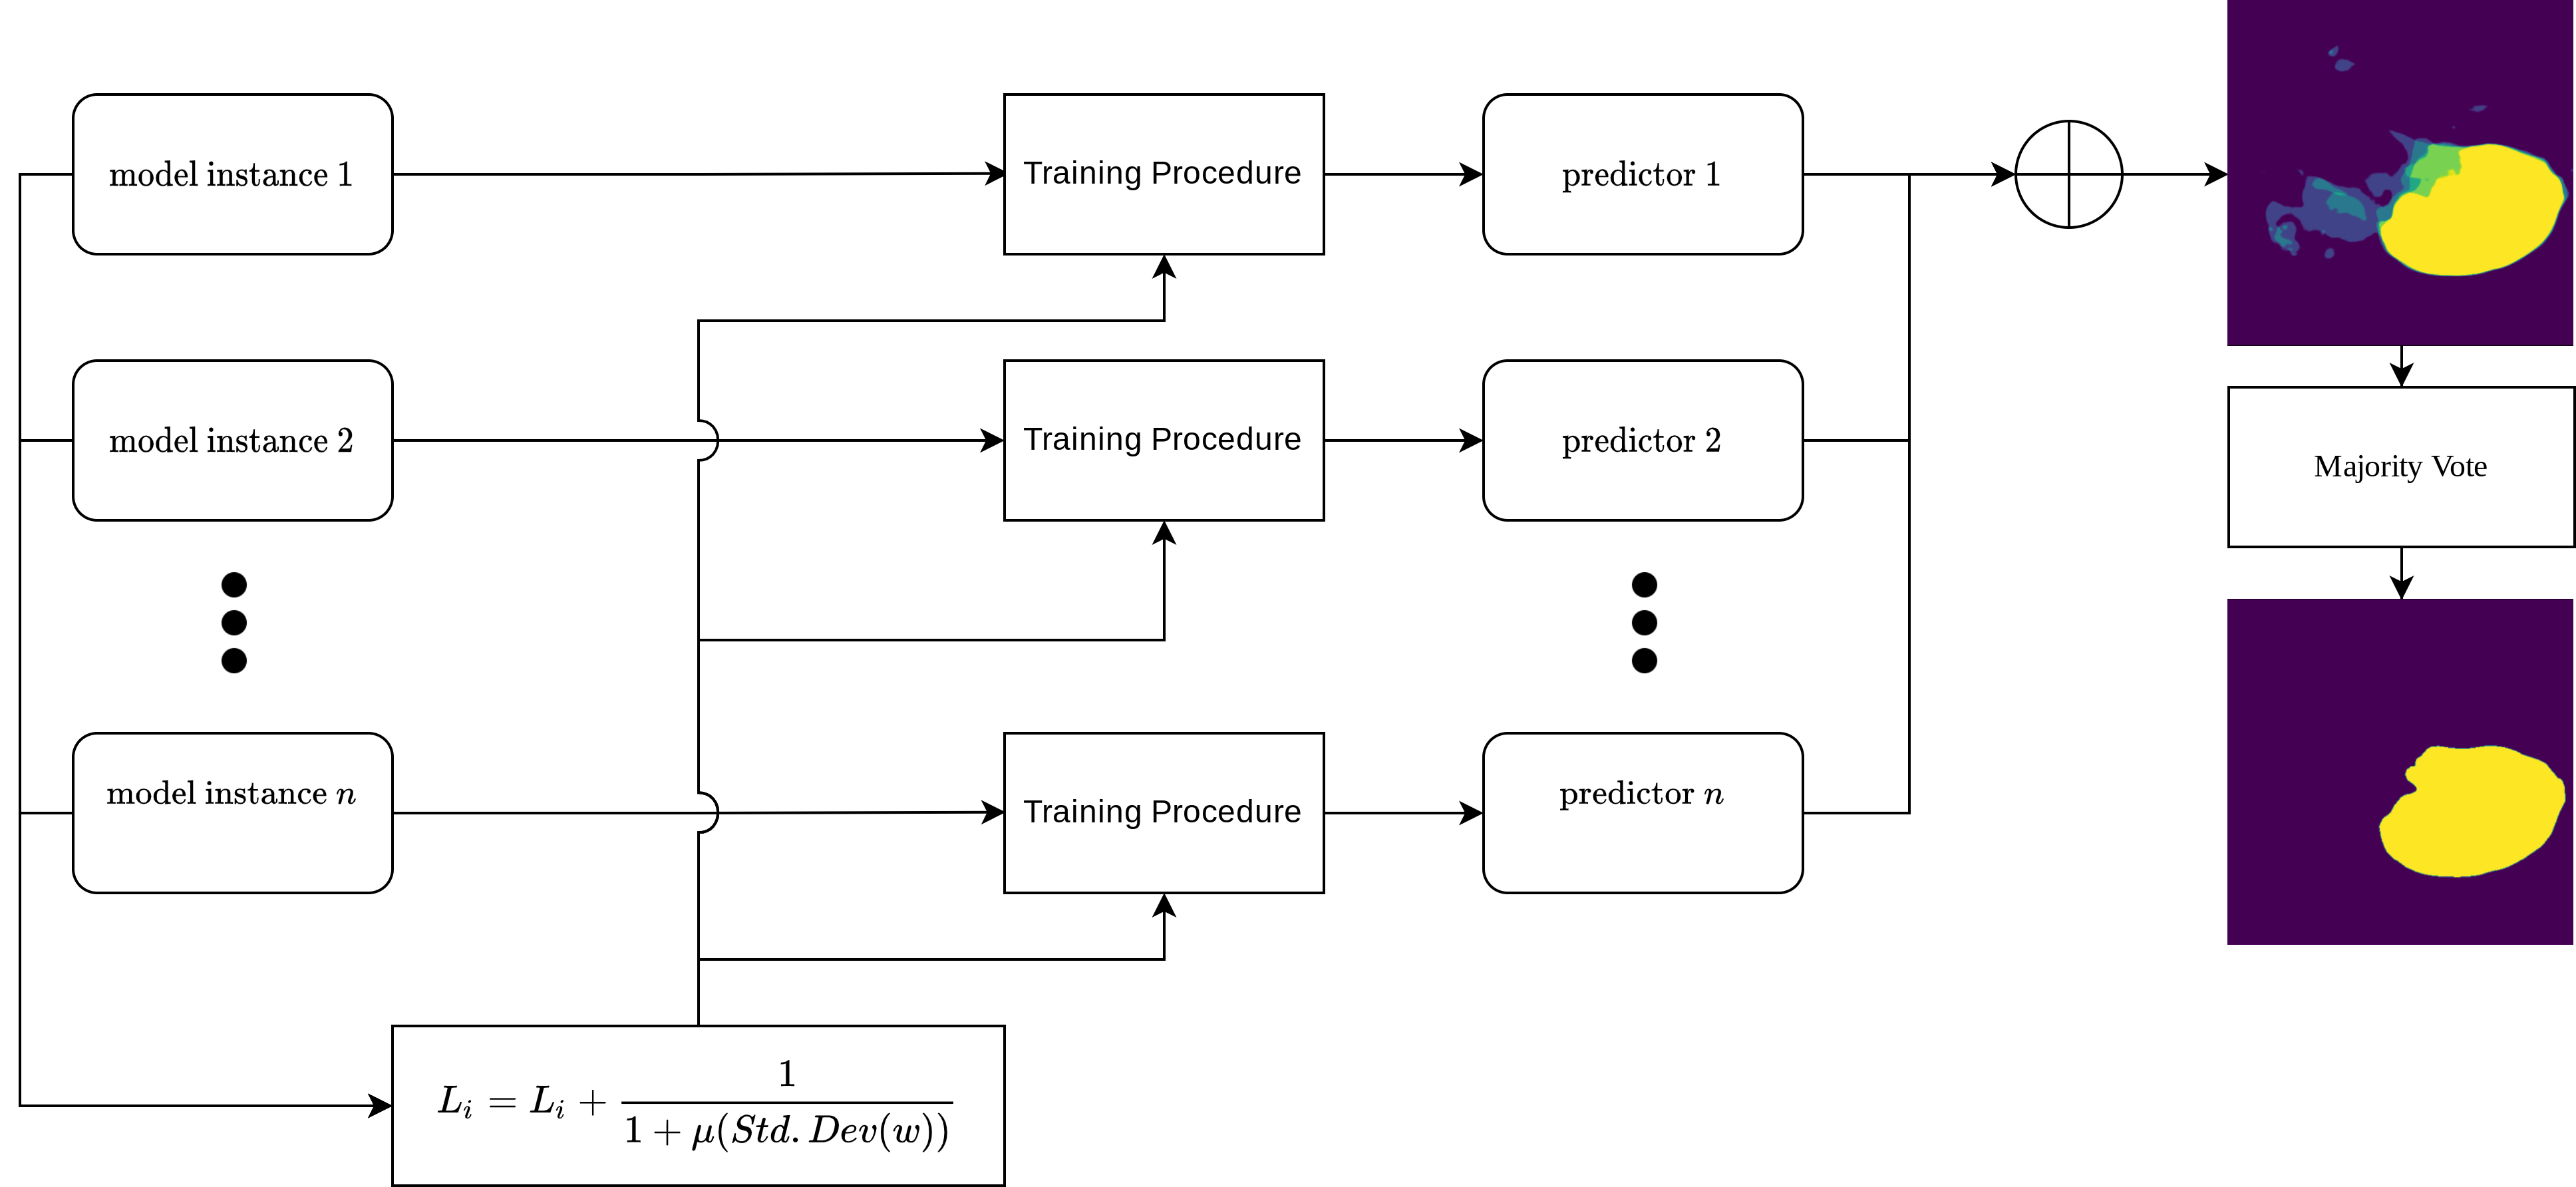
\includegraphics[width=\linewidth]{illustrations/diversity_search.png}
        \caption[Deep Diversity Search]{By adding a term corresponding to the mean standard deviation of weights, the models will learn maximally independent representations, and hence result in predictors with a larger diversity of learned features. This may mitigate underspecification to a greater extent, since this search would be less biased towards regions of the search landscape with high posterior probability.}
        \label{fig:diversity}
    \end{figure}


\section{Misc. Further work}
  This section will present a number of areas of potential further study which for various reasons could not be investigated in this thesis. 
    \subsection{Deep Preprocessing} \label{denoising}
        Consistency Training is based on increasing the support of the pipeline in a more controlled manner. Though this as established increases generalizability, it may also be possible to simply preprocess the images such that \gls{ood} transformations or artifacts are accounted for. This is acheived elsewhere using generative models - for instance a CycleGAN \cite{cyclegan}, which maps the input data between domains prior to being given to the segmentation network. One could implement a similar system using consistency training by adding a denoising network. The resulting pipeline is illustrated in \Cref{fig:preproc}
        
        \begin{figure}
            \centering
           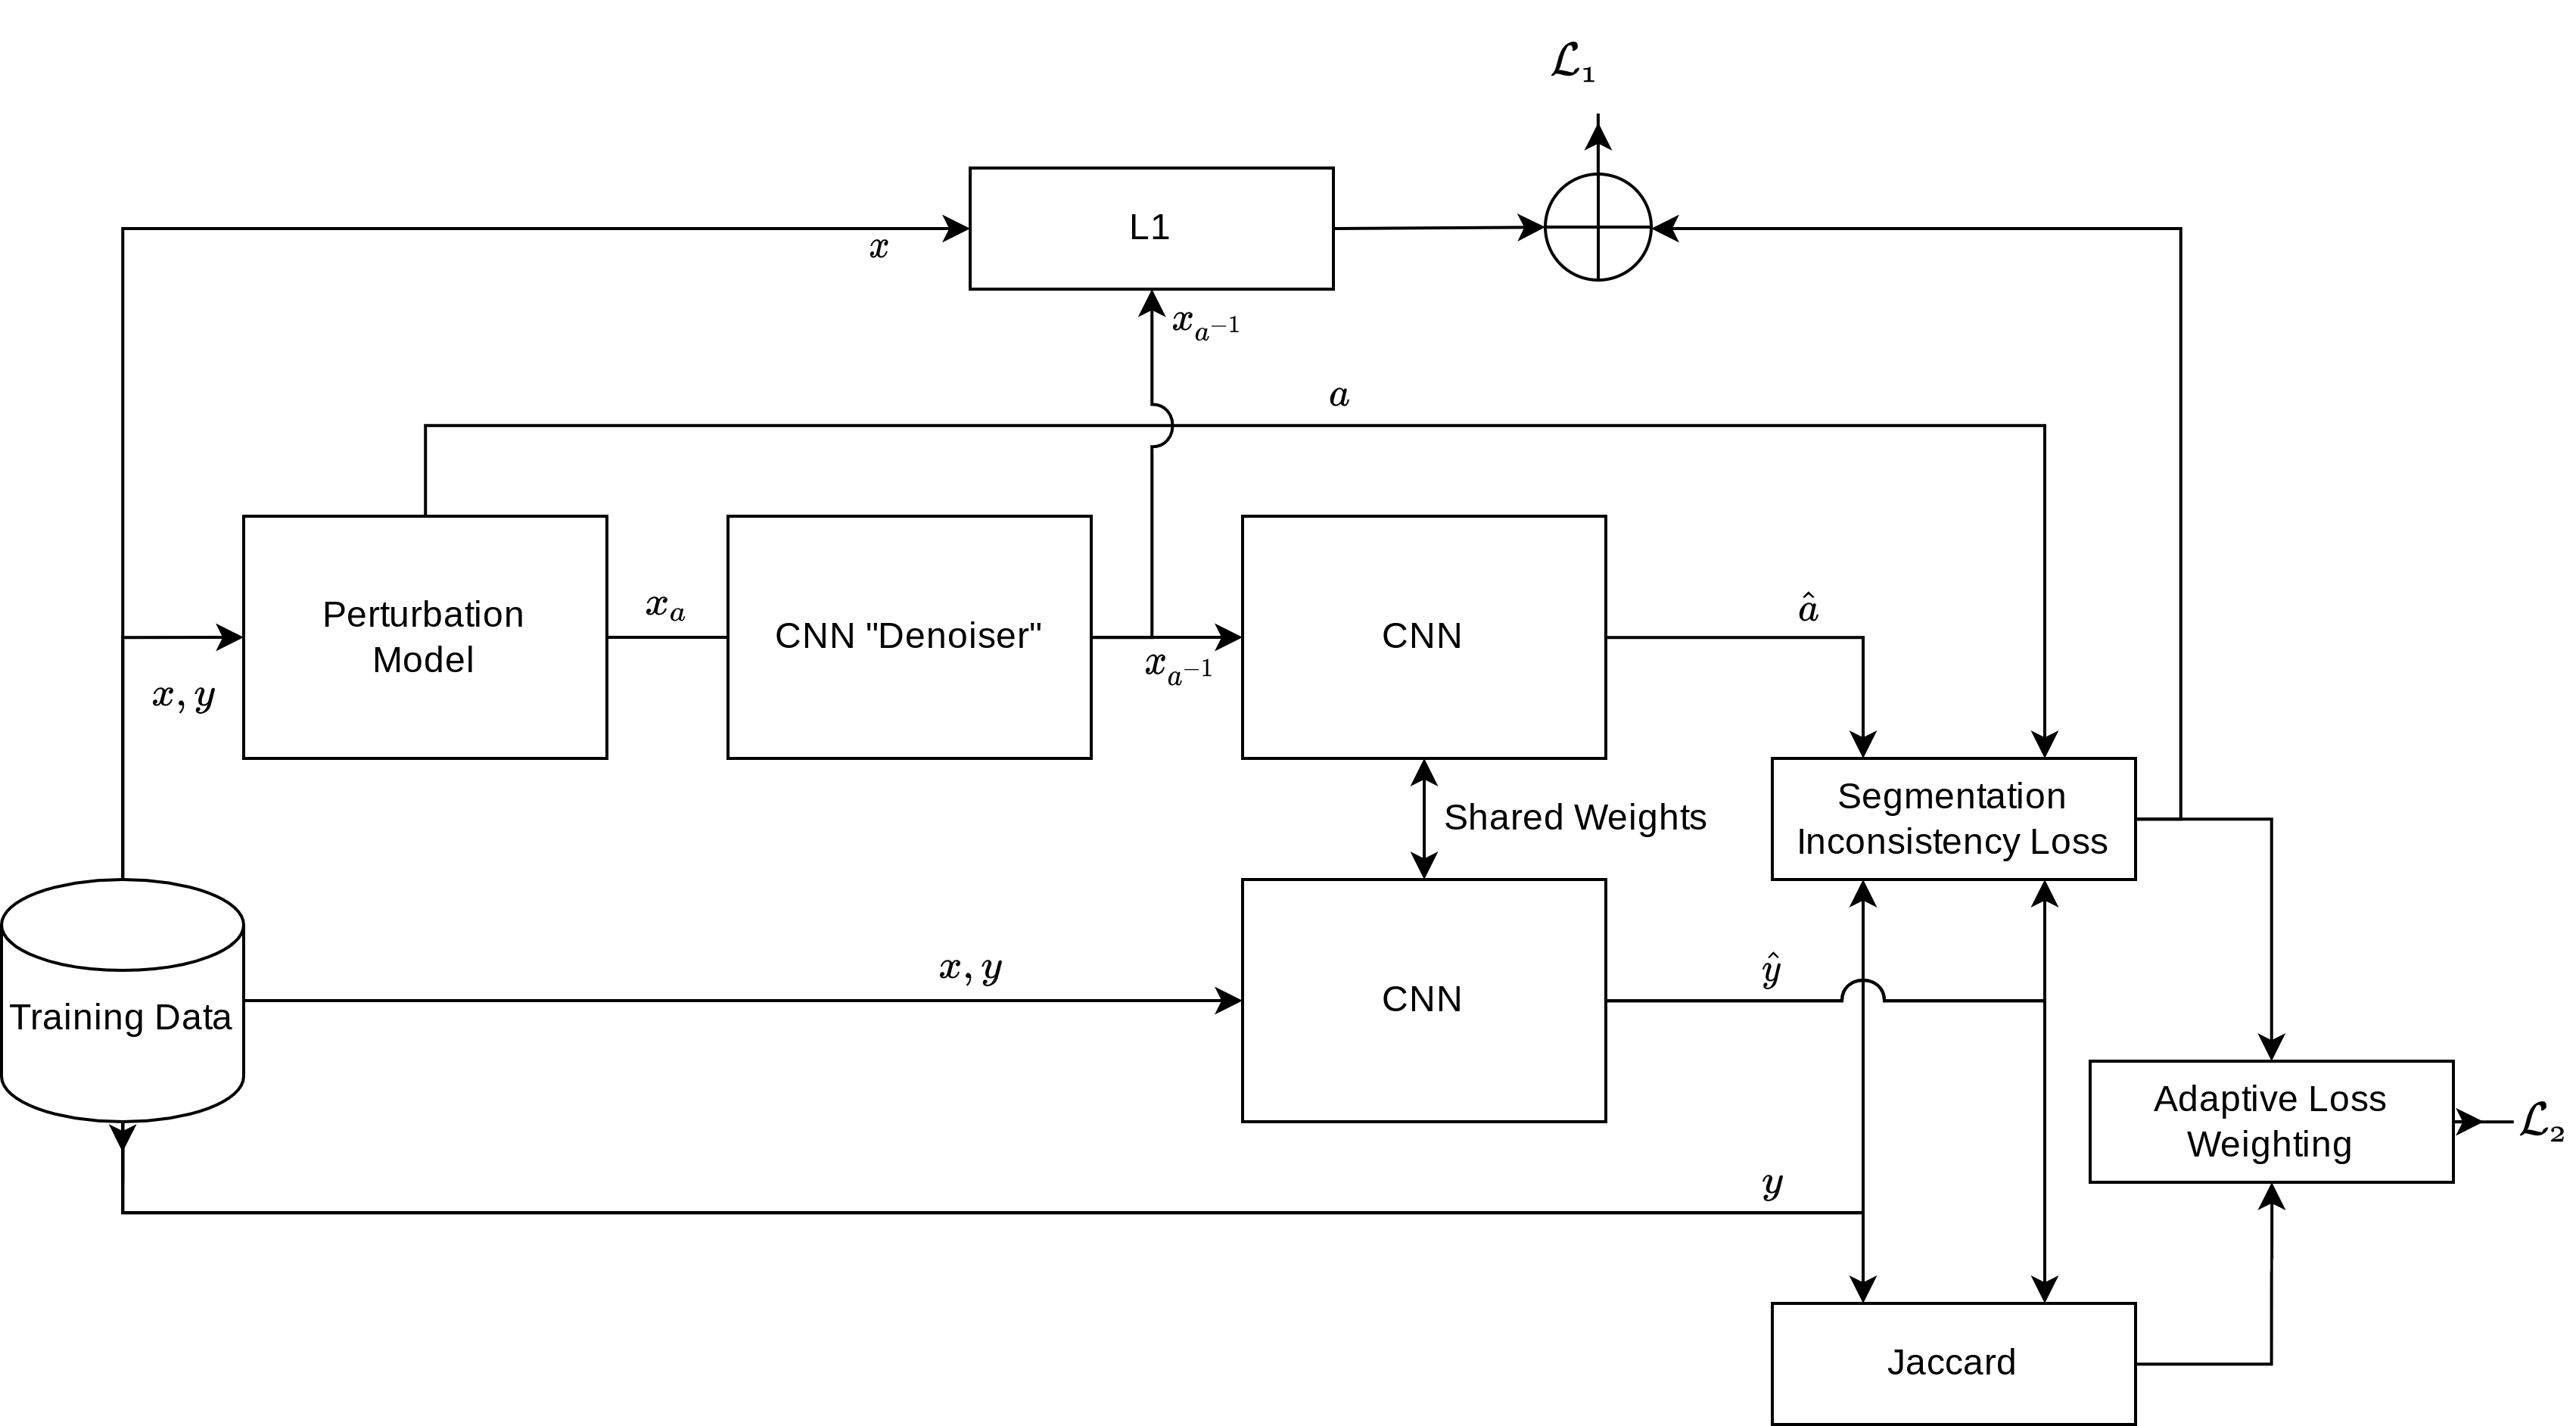
\includegraphics[width=\linewidth]{illustrations/deep_preprocessing.png}
            \caption{Consistency Preprocessing Pipeline}
            \label{fig:preproc}
        \end{figure}
        
        There are two main differences between this pipelines and more conventional deep denoising pipelines. First, the segmentation models are being trained using consistency training. Second, the denoising network is incorporating the inconsistency loss as a component of the loss function. There would in this case be two separate loss functions. In theory, this should result in the denoiser learning to counteract the characteristics of the perturbations being applied that most negatively affect the consistency and thus the generalization of the segmentation models. Moreover, even if the denoiser performs poorly, the segmentation portion should be generalizable due to consistency training, which may even be improved as a result of whatever transforms the denoising network is performing.
        
        
    \subsection{Further investigations of multitask learning}
        Multitask learning was only briefly investigated in this thesis through the dual-decoder DeepLabV3+, which as a reminder performed image reconstruction as an auxiliary tasks. Though this, interestingly, had the opposite of the intended effect - i.e, that it exhibited increased variability and reduced generalization when compared to the standard DeepLabV3+ - the results are by no means sufficiently conclusive to discredit multitask learning altogether. 
    
        Further investigating the impact of multitask learning on generalization is as such warranted. One could for instance perform a study on the impact of different tasks; perhaps image reconstruction is less conducive to generalization than something more task-adjacent, such as dimming the background or simple object detection. Depending on the results of this study, one could then also experiment with adding multiple auxiliary tasks. Investigating the variance of the latent representation in these models across multiple runs of training and comparing these to the variance in single-task models may be interesting and further the understanding of what \glspl{dnn} actually learn.
    
    \subsection{Pretraining} \label{pretraining}
        A largely neglected but nevertheless impactful aspect of the deep learning pipelines studied in this thesis is the use of pretraining. Across all the experiments performed in this thesis, every predictor was pretrained on Imagenet, with the pretrained weights being included in the segmentation-models-pytorch library \cite{smp}. Without pretraining, the models selected in this thesis exhibited IoUs of at best around 0.6 at best even on \gls{iid}, with even more significant performance gaps on \gls{ood} data. Naturally, non-pretrained networks are for this reason rarely used. However, this pretraining may play a key role in certain aspects of the behaviour observed in this thesis. In particular, pretraining may be the principle contributing factor behind the apparent ineffectiveness of multitask learning. An Imagenet pretrained encoder would, after all, perform the best when practically performing image compression.
    
\section{Summary}
This section presented a more thorough analysis and discussion of the findings as presented in \Cref{experiments}. The results were analyzed with respect to the literature, the theory as laid out in \Cref{background}, and considered in terms of viability of clinical deployment. For each experiment, the impact, limitations and potential improvements were discussed where applicable. Directions of further work were also introduced. 

Holistically, the findings in this thesis highlight that generalization remains a challenging problem, but that the development of generalizable methods is an endeavor ripe for further exploration. Consistency Training in particular seems to be a promising candidate for further research towards alleviating generalization failure. It was also shown that further foundational work is required in order to fully understand the relationship between the constituent components of the deep learning pipeline and generalizability, in particular with regards to developing sufficiently well-controlled experimental methodologies and eliminating confounding variables during comparative studies. 